\chapter{Design of DevOps Toolchain}
In the chapter, we introduce the design and implementation of our DevOps toolchain which acts as the environment of our experiments in CH5. The pipeline implementation is based on the DevOps elements we presented in Chapter 2. For experimenting that answering RQ 2, we implement two different continuous delivery pipelines design with two sets of tools respectively, one with tradition server-based tool while another one with the serverless DevOps tools from AWS. We will introduce both designs in this chapter as well.

\section{Design of Server-based DevOps Toolchain}
In section, we present our design of DevOps toolchain which based on the virtual machine.
\subsection{Architecture}
Figure \ref{fig:archjenkins} shows the architecture of our DevOps toolchain. In here we only presenting architecture on a more general level. The detailed architecture of each component will be introduced in the following sections, in both text and graph.
\par
When the developer pushes a new commit to the repository in GitHub \footnote{https://github.com/}, Github will send an HTTP POST request that contains the necessary information to the Jenkins master node. Jenkins master which triggered by the HTTP request will create a new job for this project according to the information that the HTTP request contains. The job will first pull the latest code from the git repository, then runs the docker containers with required build environment and build the project. In the end, a docker image for running the project will be created and be pushed to the container registry of AWS. Depends on the git branch that the developer committed to, the project will be deployed to a different development environment.
\par
As shown in Figure \ref{fig:archjenkins}, except version control, the whole environment is running in Amazon Web Services, 
\begin{figure}[h]
    \centering
    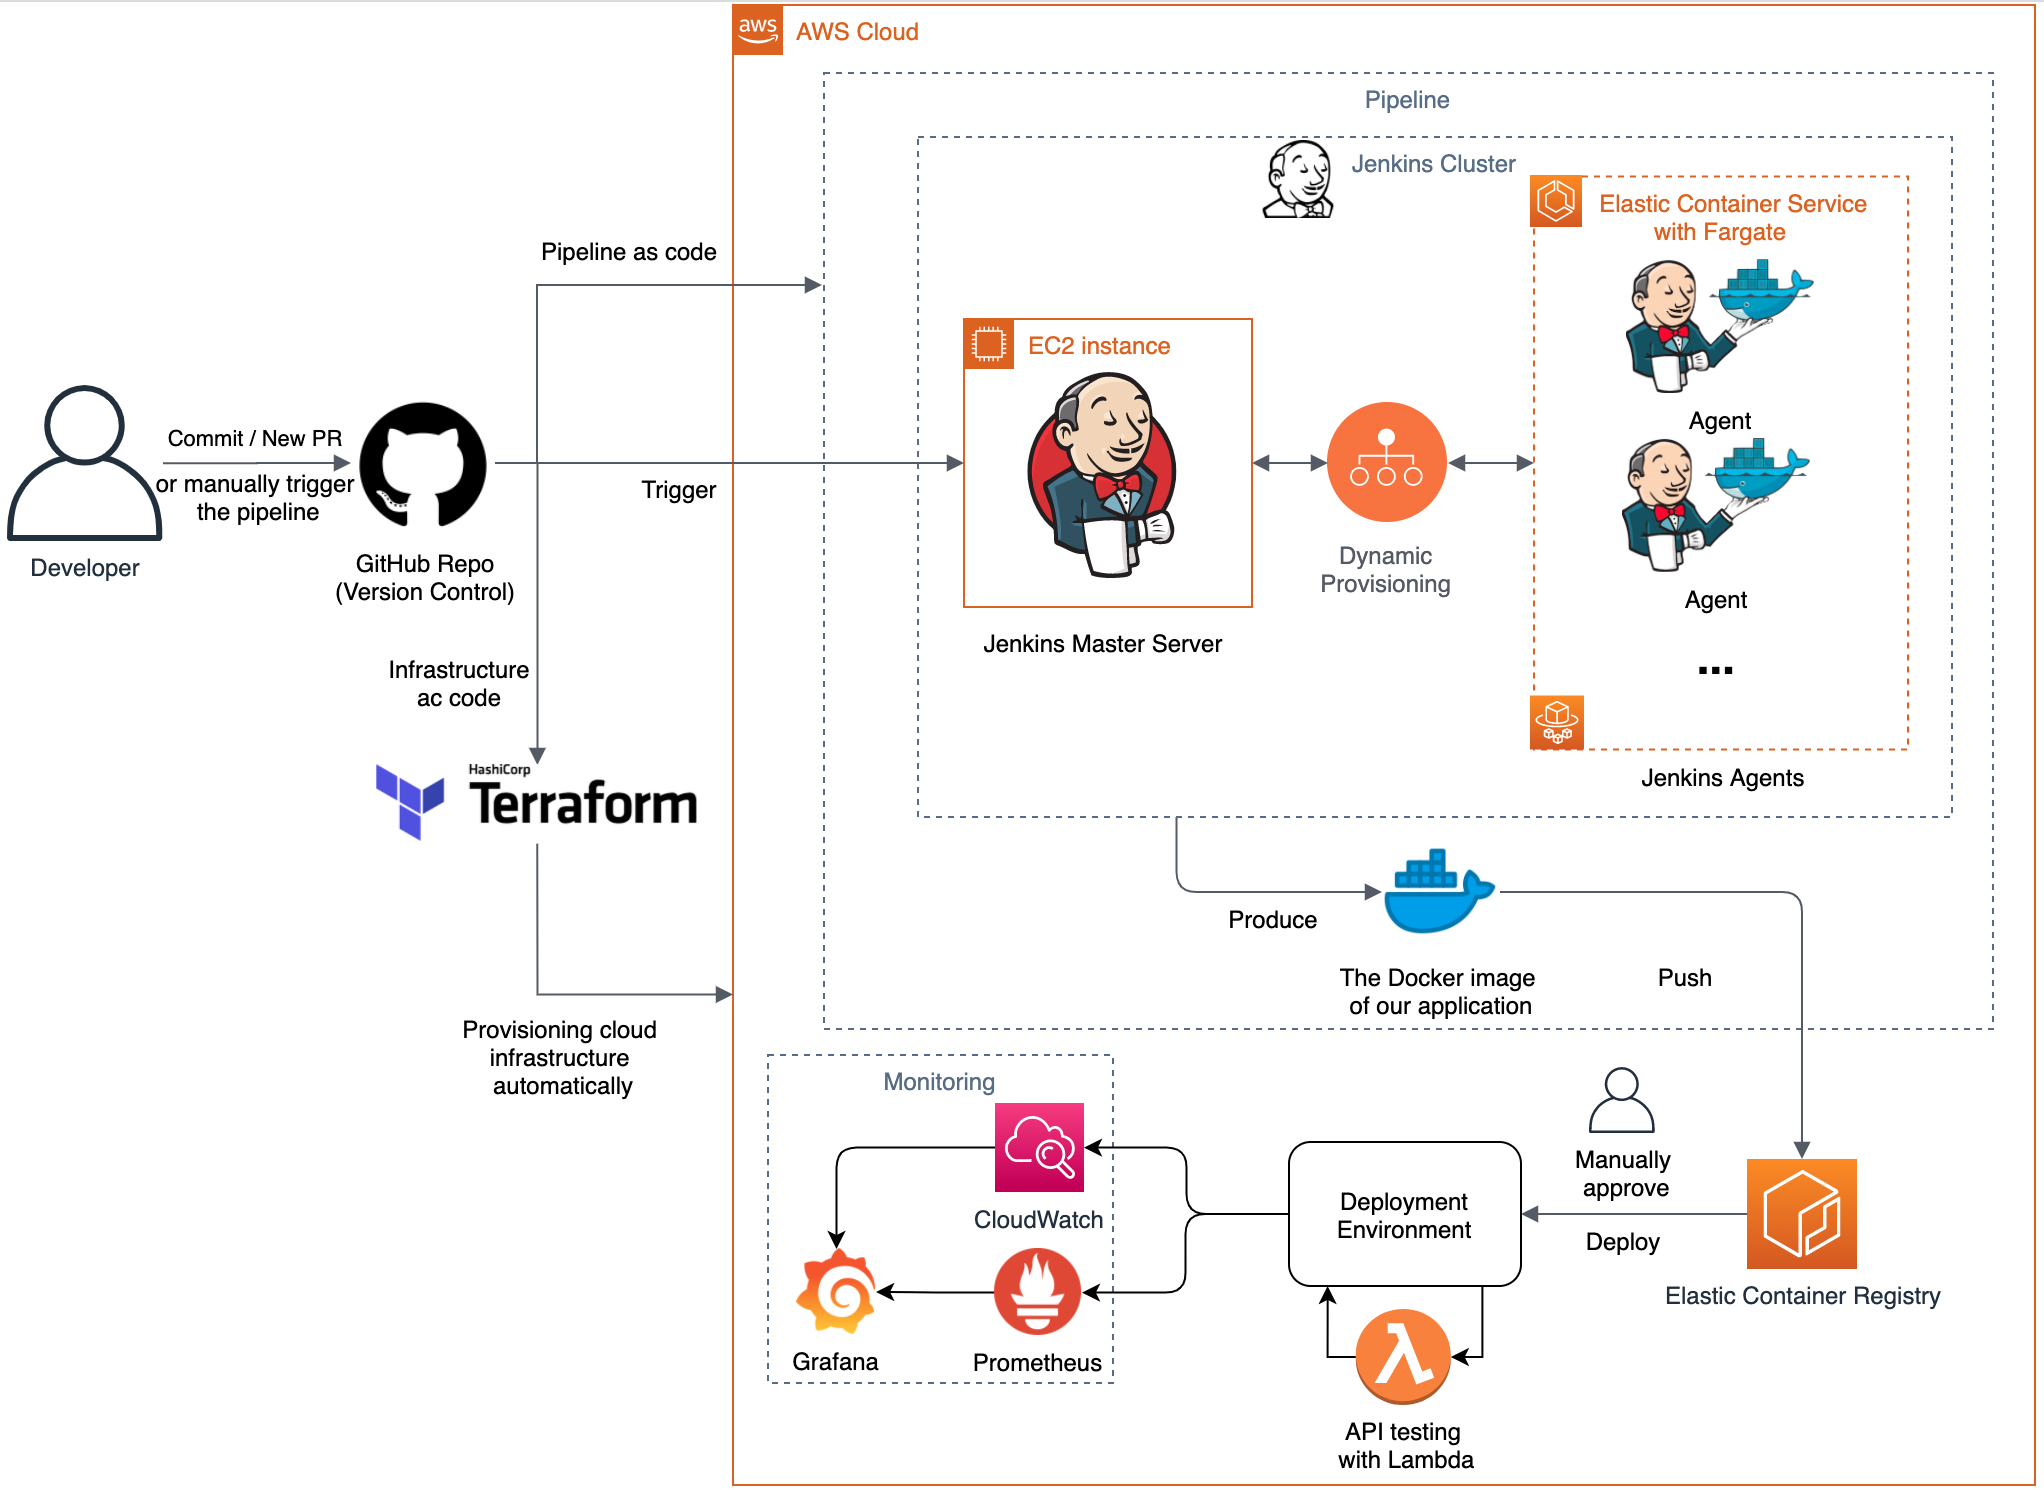
\includegraphics[width=0.99\textwidth]{pics/arch-med-jenkins.png}
    \caption{Architecture diagram of our DevOps toolchain}
    \label{fig:archjenkins}
\end{figure}
\subsection{Version Control}
\subsection{Continuous Delivery Pipeline}
\subsection{Monitoring}
\section{Design of Serverless DevOps Toolchain}
% \section{Cloud Services}
% \label{assumption}
% In this section, we will introduce several could service from CH3 that could be helpful to the DevOps toolchain. 
% //  Using services in AWS as an example, Introduces how cloud services could improve. describe services in one section
% \subsection{Managed Container Services for Distributed Builds} 

% // Describe how AWS Fargate could Help
% \subsection{Serverless computing}
% // Describe how AWS lambda could Help and why do we chose it
% \subsection{...}
